//important?//
The density profile of a dark matter halo is found to fit the NFW-profile \parencite{Navarro1996},
\begin{equation}
    \frac{\rho}{\rho_{crit}} = \frac{\delta_c}{(r/r_c)(+1+r/r_s)^2.}
\end{equation}

\epigraph{"Space is big. You just won't believe how vastly, hugely, mind-bogglingly big it is. I mean, you may think it's a long way down the road to the chemist's, but that's just peanuts to space.}{Douglas Adams, \textit{The Hitchhiker's Guide to the Galaxy}}

For that work, $f(\sigma)$ was found to be

\begin{equation}
    f(\sigma) = \frac{2}{\pi} \sigma \exp(-\sigma^2/2),
\end{equation}

but other models will give a different multiplicity function.

\subsubsection{Supermassive Black Holes}
Almost every large galaxy with a spheroidal component has a supermassive black hole (SMBH) in its center. These are black holes with masses over $10^6 M_{\odot}$ and even above $10^9 M_{\odot}$. The mass of the SMBH correlates surprisingly well with other properties of the galaxy, such as the velocity dispersion and luminosity. In the work of \cite{Ferrarese2000} the mass of the SMBH was found to be related to the velocity dispersion of the bulge component of the galaxy as a power law


\begin{equation}
    M_{BH} \propto \sigma^{\alpha},
\end{equation}

with power law index $\alpha = 4.8 \pm 0.5$ The correlation 
%describe how!

This is surprising because the SMBH only has a gravitational influence within a very small radius compared to the entire galaxy, which suggests that the SMBH evolves along with the galaxy and that their formation is linked. In fact, it seems very likely that these gigantic black holes play a vital role in galaxy evolution, and are a central component of the galaxy as a whole.


\subsection{SMBH relations}
In Figure \ref{bh_res} the SMBH-mass and velocity dispersion for TNG100 is shown, along with the best fit functions from \cite{Ferrarese2000} and \cite{Tundo2007}.

\begin{figure}
    \centering
    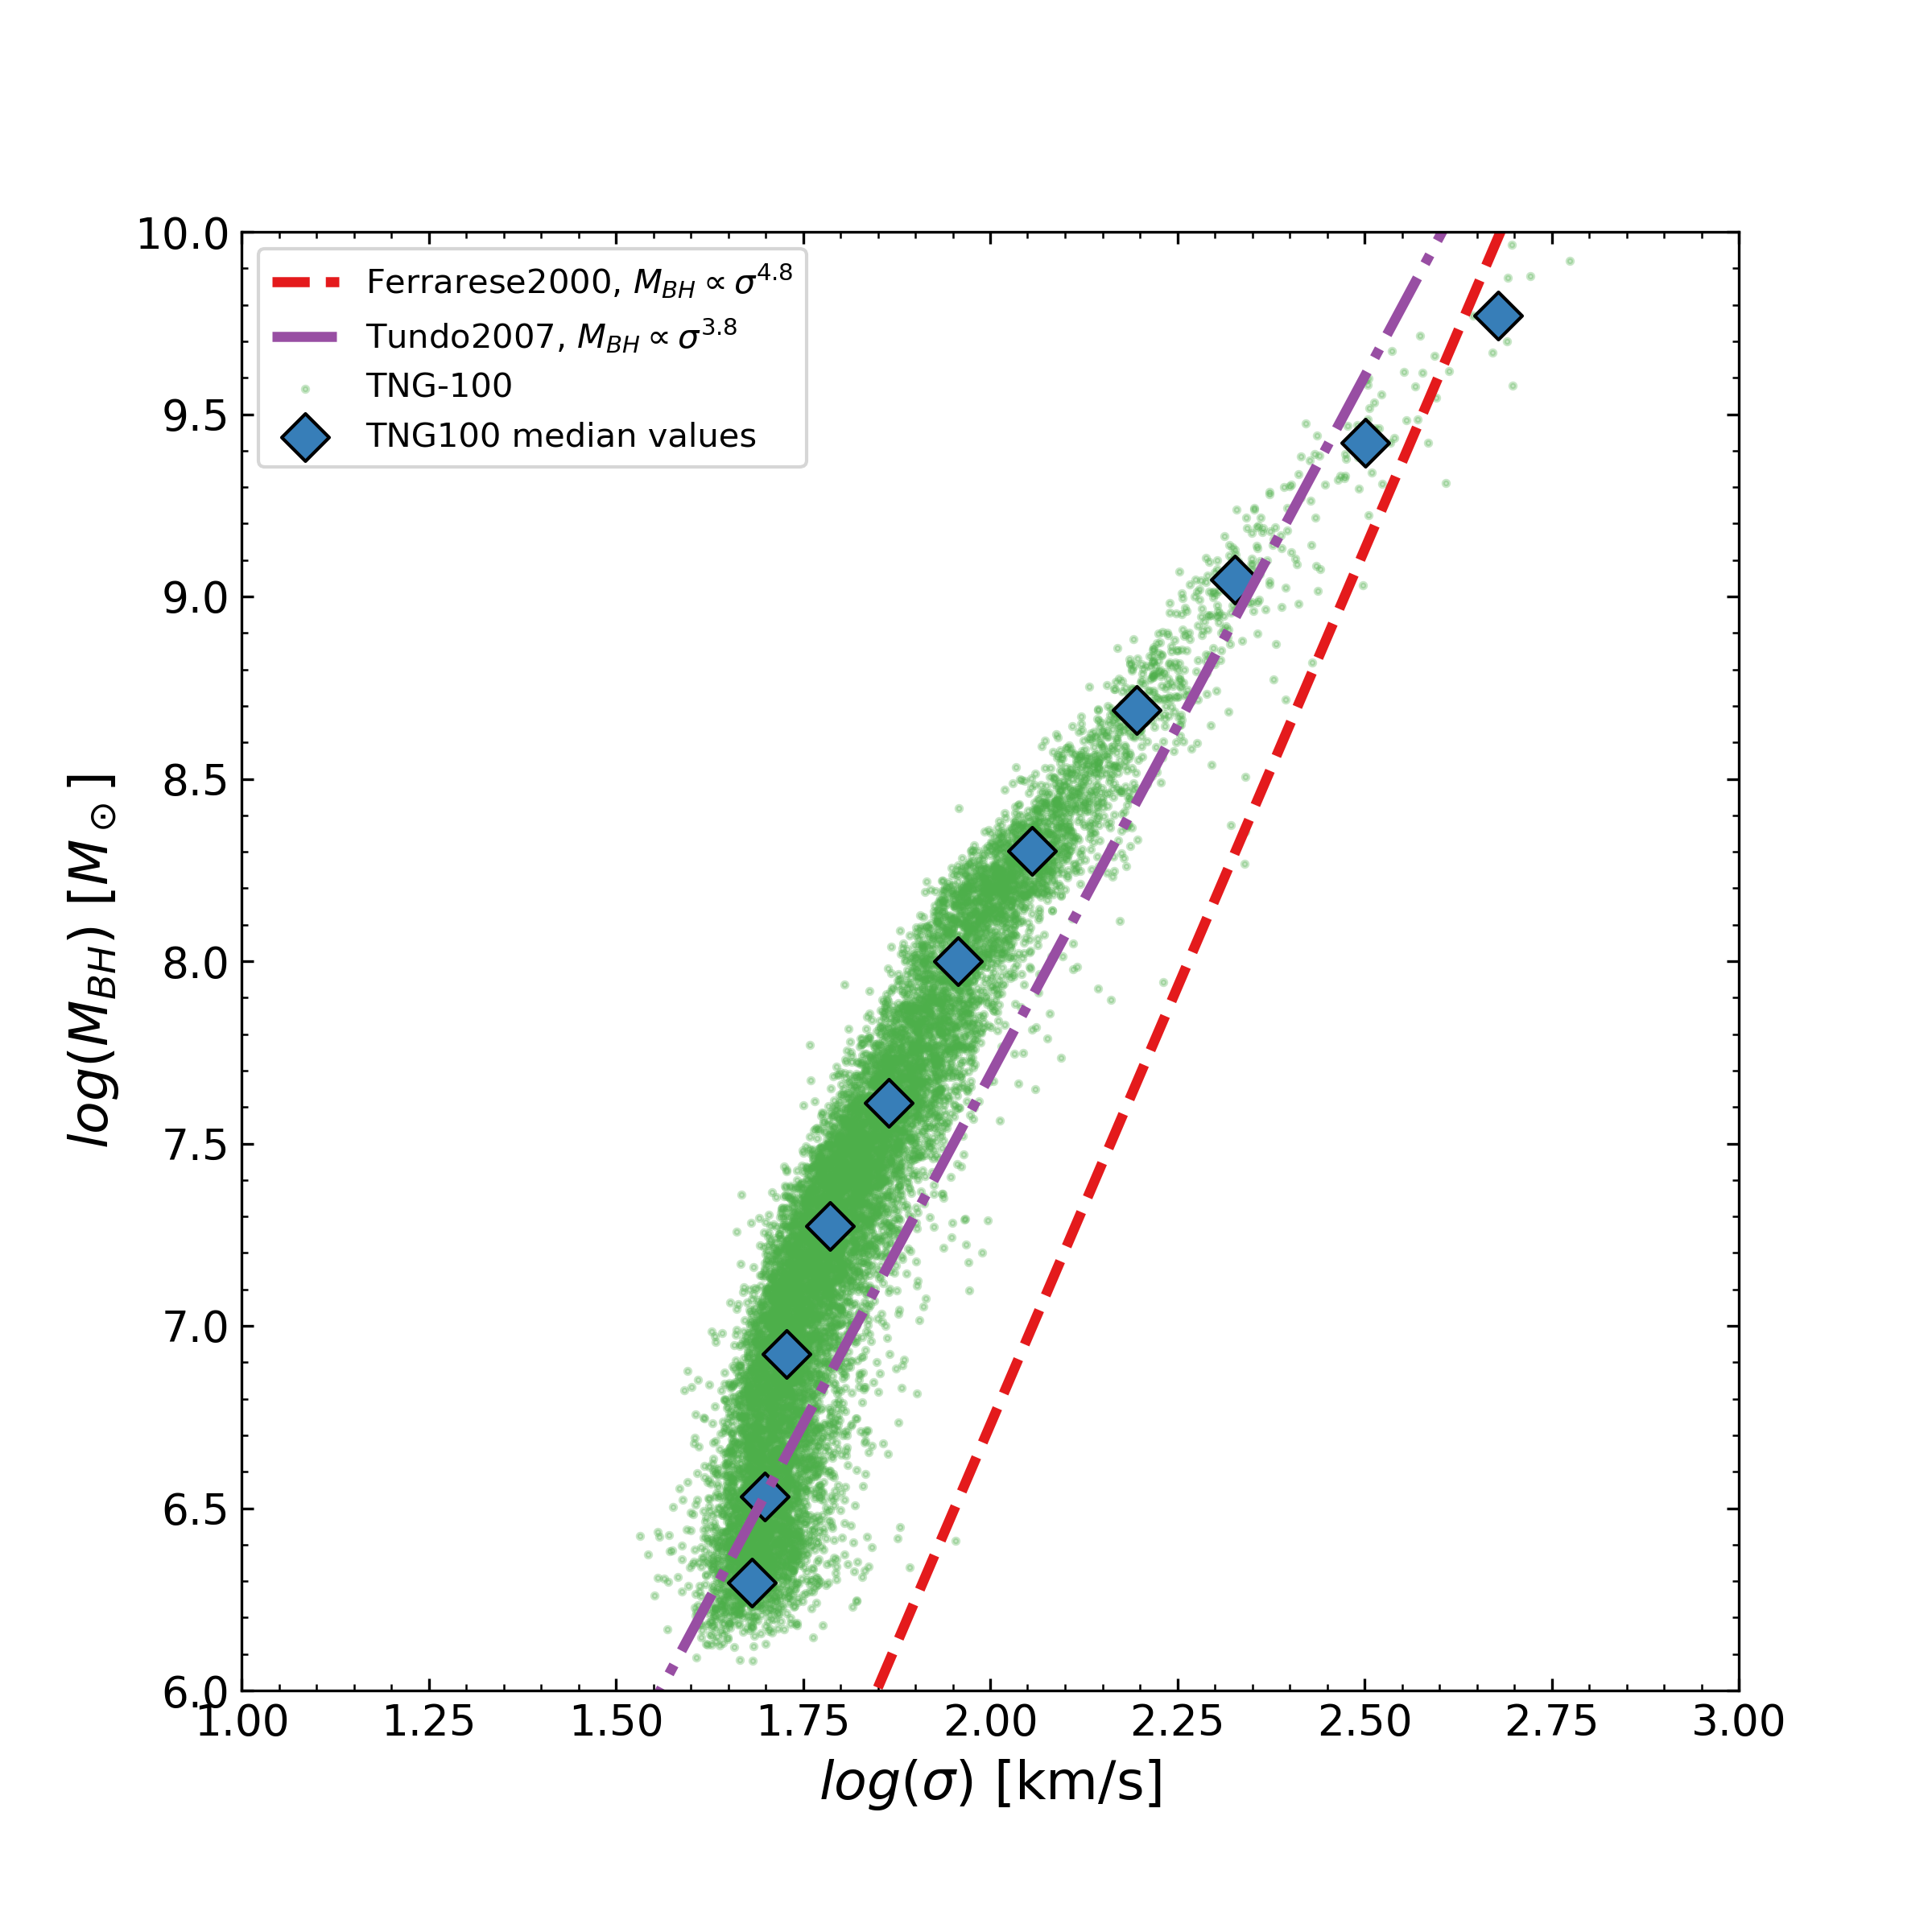
\includegraphics[width=0.9\textwidth]{images/results_mass_BH_sigma.png}
    \caption{}
    \label{bh_res}
\end{figure}


IllustrisTNG-distances are given as comoving distances. Comoving and proper distances are two measurements of distance used in cosmology and are closely linked. The comoving distance between two particles that are only moving with the Hubble flow is constant. The proper distance factors in the expansion of the universe, and so the distance between the two particles would increase with time. For $z=0$, the proper and comoving distance of two objects are the same so no conversion is needed.



\begin{table}
\begin{center}
\caption{The different filters studied in this work. TNG has photometric data available for U,B,V,K,u,g,r,i,z filters.}
\label{filters}
\begin{tabular}{ l| c c c c } 
 \hline
 \hline
   & U & g & r & i \\
 \hline
 System  & UBV & SDSS & SDSS & SDSS \\
 Wavelength (nm) & 364 & 475 & 622 & 763 \\
 \hline
\end{tabular}
\end{center}
\end{table}